\chapter{Tổng quan}
\label{ch:tongquan}
\minitoc

%\newpage

Các tia bức xạ $\gamma$ sẽ được ghi nhận thông qua quá trình tương tác với vật chất. Đặc tính điện từ của các tia bức xạ $\gamma$ cho phép các tia bức xạ này có thể tương tác với các điện tử. Nguyên lý ghi nhận các tia bức xạ $\gamma$ dựa trên hiện tượng ion hóa: Các tia bức xạ $\gamma$ sẽ chuyển một phần hoặc toàn bộ năng lượng cho các điện tử. Các điện tử tự do được tạo thành trong quá trình này sẽ tương tác với các nguyên tử gần đó để tạo các điện tử thứ cấp. Các điện tử này được ghi nhận để xác định năng lượng của các tia $\gamma$. Kết quả của việc ghi nhận là một xung điện tỷ lệ với năng lượng của tia $\gamma$ đã  bị mất trong môi trường do quá trình tương tác.\xdyIndex{0 gamma@$\gamma$}

\section{Hiệu ứng quang điện}
\xdyIndex{quang điện}
Ở năng lượng thấp ($<$ 200 keV), tương tác giữa photon với một tinh thể Germanium được thực hiện thông qua hiệu ứng quang điện. Trong trường hợp này năng lượng của photon được hấp thụ hoàn toàn bởi tinh thể Germanium. Xác suất tương tác được tính một cách gần đúng theo công thức \cite{bib_Knoll, bib_ghinhanbucxa, bib_vatlyhatnhanungdung}:

%, bib_ghinhanbucxa, bib_vatlyhatnhanungdung}:

\begin{equation} 
P_{ph}\approxeq k\cfrac{Z^{n}}{(h\nu)^{3.5}}
\label{equ:huquangdien}
\end{equation}

Trong đó, giá trị của $n$ thay đổi từ 4 đến 5 tương ứng với khoảng năng lượng của photon từ 0 đến 3 MeV, $h\nu$ \nomenclature{$\nu$}{Tần số sóng điện từ} và $Z$ lần lượt là năng lượng của photon và số hiệu nguyên tử của Germanium.

\section{Hiệu ứng Compton}
\xdyIndex{Compton}
\xdyIndex{hiệu ứng}
Công thức \ref{equ:huquangdien} được áp dụng cho các photon có năng lượng thấp, tuy nhiên khi photon có năng lượng lớn hơn ($\approx$ 200 keV đến 8 MeV), hiệu ứng Compton sẽ chiếm ưu thế. Trong quá trình này, một photon có năng lượng $h\nu_{0}$ sẽ thực hiện tương tác không đàn hồi với một điện tử\footnote{Cần phân biệt giữa tán xạ Compton với tán xạ Rayleigh trong đó các tia $\gamma$, sau khi tương tác với một điện tử, thay đổi hướng chuyển động và không mất đi năng lượng.}. Một phần năng lượng của photon bị mất do tương tác với điện tử và các tia $\gamma$ sau  đó sẽ tán xạ dưới một góc $\theta$ \nomenclature{$\theta$}{Góc tán xạ} so với hướng ban đầu với năng lượng $h\nu$. Theo định luật bảo toàn năng lượng và động lượng ta có:
%
\begin{equation}
h\nu=\cfrac{m_{0}c^{2}\alpha}{1+\alpha(1-\cos{\theta})}
\end{equation}

Trong đó $\alpha=\cfrac{h\nu_{0}}{m_{0}c^{2}}$, $m_{0}$ là khối lượng của điện tử. Động năng của điện tử $(T=h\nu_{0}-h\nu)$ đạt cực 	đại nếu $\theta=\pi$. Tiết diện phản ứng vi phân tính trên một điện tử $\sigma_{e}$ \nomenclature{$\sigma_e$}{Tiết diện phản ứng vi phân trên một điện tử} với một góc khối $\Omega$ được thể hiện bằng công thức Klein-Nishina \cite{bib_Klein}:

\xdyIndex{tiết diện}
\begin{equation}
\cfrac{d \sigma_{e}}{d \Omega} = \cfrac{r_{0}^{2}}{2} 
\biggl\{
 \cfrac{1}{[1+\alpha(1-cos\theta)]^{2}}
 \biggl [
	1+cos^{2}\theta+\cfrac{\alpha^{2}(1-cos\theta)^{2}}{[1+\alpha (1-cos\theta)]}
 \biggr ]
\biggr\}
\end{equation}

trong đó $r_{0}$\nomenclature{$r$}{Bán kính tán xạ của điện tử} bán kính của điện tử. 

Các giá trị tiết diện phản ứng vi phân đối với các photon\xdyIndex{photon} có năng lượng\xdyIndex{năng lượng} từ 0.2 MeV đến 2 MeV (khoảng giá trị đặc trưng được sử dụng khi nghiên cứu phổ các tia bức xạ $\gamma$) được thể hiện trên Hình \ref{fig:klein}. Các giá trị đã được chuẩn hóa theo giá trị tiết diện phản ứng cực đại được tính theo hướng của photon. Ở mức năng lượng cao ($\geq$ 1 MeV) hầu hết các tia bức xạ $\gamma$ tán xạ ở một góc rất nhỏ. Tuy nhiên, ở năng lượng thấp, các tia $\gamma$ có thể tán xạ ở các góc lớn hơn.\xdyIndex{góc tán xạ}\xdyIndex{động năng} 

\begin{figure}[!h]
\centering
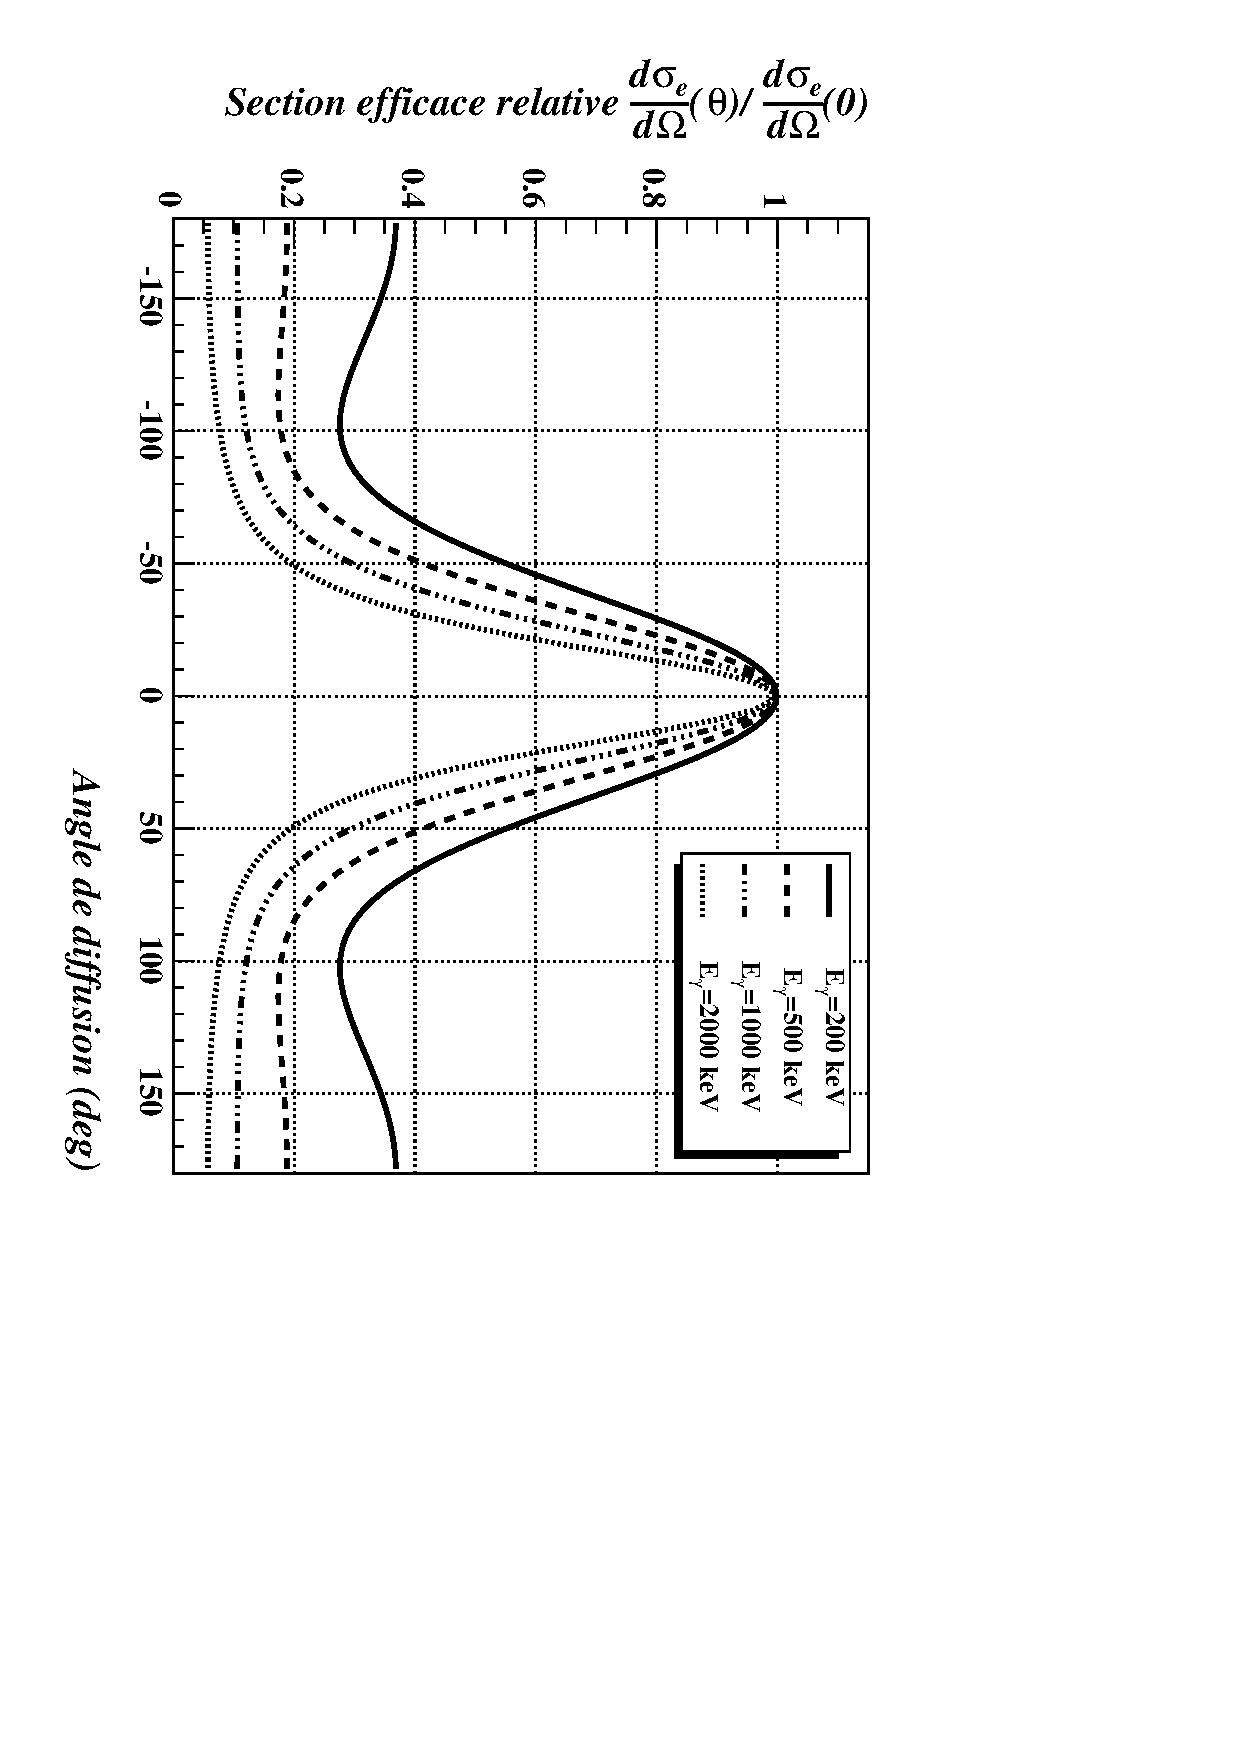
\includegraphics[height=0.8\textwidth,angle = 90.0 ]{figure/fig_cosolythuyet/klein.pdf}
\caption{Tán xạ Compton của các tia bức xạ $\gamma$ theo công thức Klein-Nishina cho khoảng năng lượng từ 200 keV đến 2 MeV.}
\label{fig:klein}
\end{figure}

Ở mức năng lượng lớn hơn 1.022 MeV, xác suất của quá trình tạo cặp sẽ tăng dần và sẽ đạt giá trị lớn hơn giá trị xác suất của quá trình tán xạ Compton khi năng lượng của photon tới lớn hơn 8 MeV. Hiệu ứng tạo cặp gắn liền với hiện tượng biến đổi từ một tia bức xạ $\gamma$ thành một 		điện tử và một positron có động năng lần lượt là $T_{-}$ và $T_{+}$. Mối liên hệ giữa động năng của các hạt được tạo thành với năng lượng của photon ban đầu được biểu thị bằng công thức sau:

\section{Hiệu ứng tạo cặp}
\xdyIndex{tạo cặp}
Ở mức năng lượng lớn hơn 1.022 MeV, xác suất của quá trình tạo cặp sẽ tăng dần và sẽ đạt giá trị lớn hơn giá trị xác suất của quá trình tán xạ Compton khi năng lượng của photon tới lớn hơn 8 MeV. Hiệu ứng tạo cặp gắn liền với hiện tượng biến đổi từ một tia bức xạ $\gamma$ thành một 		điện tử và một positron có động năng lần lượt là $T_{-}$ và $T_{+}$. Mối liên hệ giữa động năng của các hạt được tạo thành với năng lượng của photon ban đầu được biểu thị bằng công thức sau:

\begin{equation}
h\nu_{0} = T_{-} + T_{+} + 2m_{0}c^{2}
\end{equation}

$h\nu_{0}$ là năng lượng của photon, $m_{0}$\nomenclature{$m$}{ Khối lượng điện tử} là khối lượng của một điện tử. Sự biến đổi trên chỉ có thể được thực hiện ở gần một hạt nhân hoặc gần một điện tử để đảm bảo 	  định luật bảo toàn mô men động lượng được thỏa mãn. Tiết diện phản ứng của quá trình tạo cặp tỷ lệ với $Z^{2}$. Positron tạo thành từ phản ứng này sẽ hủy cặp với một điện tử khác để tạo ra hai tia bức xạ $\gamma$ có năng lượng 511 keV và được phát ra theo hai hướng đối lập.

\renewcommand\bibname{Tài liệu tham khảo chương \thechapter}
\bibliographystyle{ieeetr}
\bibliography{bibtex/biblio} %put path to the Bib from where the BibtexRun.bat is located 